\documentclass[tikz]{standalone}
\usepackage{amsmath}
\definecolor{bgcol}{HTML}{171D2B}
\definecolor{accent}{HTML}{F7B538}
\definecolor{setcol}{HTML}{7DA2C9}
\pagecolor{bgcol}
\begin{document}
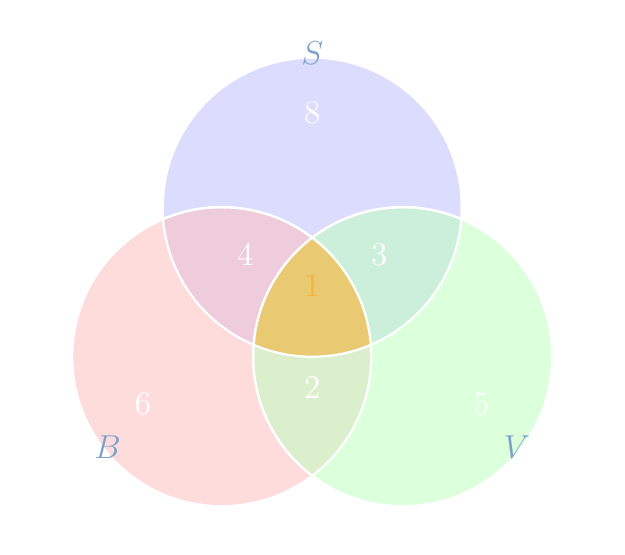
\begin{tikzpicture}[scale=1.0, color=white, font=\large]
  % Diagram Venn tiga himpunan: sepak bola (S), basket (B), voli (V)
  % Survei 40 siswa kelas VII
  %   hanya S = 8, hanya B = 6, hanya V = 5
  %   S dan B saja = 4, S dan V saja = 3, B dan V saja = 2
  %   ketiganya = 1, tidak satu pun = 11
  % Tiga pusat membentuk segitiga, jari-jari sama
  \coordinate (A) at (0, 1.15);
  \coordinate (B) at (-1.15, -0.75);
  \coordinate (C) at (1.15, -0.75);

  % Persegi panjang semesta
  \draw[thick] (-3.6, -2.9) rectangle (3.6, 3.3);
  \node[anchor=south west] at (-3.4, 2.9) {$S$};

  % Ketiga lingkaran dengan warna isi berbeda
  \draw[thick, fill=blue!25, fill opacity=0.55]  (A) circle (1.9);
  \draw[thick, fill=red!25, fill opacity=0.55]   (B) circle (1.9);
  \draw[thick, fill=green!25, fill opacity=0.55] (C) circle (1.9);

  % Irisan tiga diwarnai tegas: potong dengan A, lalu dengan B,
  % kemudian isi lingkaran C di dalam potongan itu
  \begin{scope}
    \clip (A) circle (1.9);
    \clip (B) circle (1.9);
    \fill[accent, fill opacity=0.6] (C) circle (1.9);
  \end{scope}

  % Gambar ulang garis lingkaran supaya tetap tegas
  \draw[thick] (A) circle (1.9);
  \draw[thick] (B) circle (1.9);
  \draw[thick] (C) circle (1.9);

  % Label himpunan di luar lingkaran
  \node[setcol] at (0, 3.1) {$S$};
  \node[setcol] at (-2.6, -1.9) {$B$};
  \node[setcol] at (2.6, -1.9) {$V$};

  % Angka: hanya satu himpunan
  \node at (0, 2.35) {$8$};
  \node at (-2.15, -1.35) {$6$};
  \node at (2.15, -1.35) {$5$};
  % Angka: irisan dua himpunan
  \node at (-0.85, 0.55) {$4$};
  \node at (0.85, 0.55) {$3$};
  \node at (0, -1.15) {$2$};
  % Angka: irisan tiga himpunan
  \node[accent] at (0, 0.15) {$1$};
  % Angka: di luar ketiga lingkaran
  \node at (3.0, 2.6) {$11$};
\end{tikzpicture}
\end{document}
